\documentclass[a4paper, 10.5pt, twoside]{jreport}

% include
\usepackage{gra_yasuda}
\usepackage{lscape}
\usepackage{graphicx}
\usepackage{here}
\usepackage{color}
\usepackage{amsmath}
\usepackage{subfig}
\usepackage{tascmac}
\usepackage{url}
\usepackage{ascmac}
\usepackage{booktabs}
\usepackage{otf}
\usepackage{comment}



%タイトル
\title{心理的効果を用いた人間とエージェントの繰り返し交渉戦略}
\etitle{Repetitive negotiation strategy of human and agent \\ using psychological effect}

%名前
\author{松下 昌悟}
\eauthor{Shogo MATSUSHITA}

%入学年度
\enteryear{2017}
%卒業年度
\graduateyear{2018}

%学籍番号
\studentnumber{17268508}

%提出日
\date{平成30年1月31日}

\begin{document}

%ここで行ピッチを指定
%フォントを変えるとサイズがリセットされてしまうので注意
\setlength{\baselineskip}{8truemm}


%ここから内容

% Chapter 4
\chapter{予備実験}\label{cha:4}

\section{目的と概要}
提案手法に用いる各種パラメータを決定することを目的としてエージェント同士での交渉を行う実験を行う.
具体的には提案手法の戦略を適用した8つのエージェントと予備実験用の戦略を適用したエージェントでそれぞれ交渉を行う.
本実験では,提案手法の戦略を適用したエージェントの個人効用が高いほど良いパラメータであると評価する.

\section{実験設定}
本実験では,各論点が0\sim 5の計6つの選択肢を有する,4つの論点について交渉を行う.

本実験で用いるドメインの詳細およびパラメータを表\ref{tab:pre_domain},表\ref{tab:pre_para}にそれぞれ示す.

\begin{table}[htb]
  \begin{center}
    \caption{予備実験で用いるドメイン}
    \label{tab:pre_domain}
    \begin{tabular}{|c|c|c|c|} \hline
      論点数 & 各論点の選択肢数 & 繰り返し回数 & 留保価格 \\ \hline \hline
      4 & 6 & 5 & 4 \\ \hline
    \end{tabular}
  \end{center}
\end{table}

\begin{table}[htb]
  \begin{center}
    \caption{予備実験で用いるパラメータ}
    \label{tab:pre_para}
    \begin{tabular}{|c|c|c|c|c|c|} \hline
      & \alpha の初期値 & \alpha の増分 & \beta の初期値 & \beta の増分 & \alpha の更新回数 \\ \hline \hline
      取りうる値 & 0.0 \sim 8.0 & 0.5 \sim 4.0 & 0.0 \sim 8.0 & 0.5 \sim 4.0 & 1 \sim 10 \\ \hline
      刻み幅 & 1.0 & 0.5 & 1.0 & 0.5 & 1 \\ \hline
      取りうる値の総数 & 9 & 8 & 9 & 8 & 10 \\ \hline
    \end{tabular}
  \end{center}
\end{table}

本実験では表\ref{tab:pre_domain}に示したように,1セット5回の交渉を行う.
各論点の価値は1セットごとにランダムに変化させるが,各論点の価値は$1 \sim 4$の間の整数値で重複はない.
また,提案手法のエージェントにとって価値が一番高いものは予備実験用のエージェントにとって一番価値が低いといったように,一方にとって価値が高いものはもう一方にとって価値が低くなるように設定する.
各論点の価値の例を表\ref{tab:pre_value}に示す.
論点1を例にとると,提案手法のエージェントにとっての価値は4であり,一番価値がある論点となる.
対して予備実験用のエージェントにとっての価値は1であり,一番価値がない論点となる.
本実験では各論点に対して0から5の計6つの選択肢が存在し,提案手法のエージェントと予備実験用のエージェントは同一の論点において選択肢の値の合計は5以下でなければならない.例として,提案手法のエージェントが論点1において選択肢3を選択した場合,予備実験用のエージェントは論点1において選択肢3,4,5を選択することはできない.最終的に全ての論点において両エージェントの選択肢数の合計が5となった提案(FullOffer)が受諾された場合,交渉は終了する.時間内に全ての論点における両エージェントの選択肢数の合計が5にならなかった場合,両エージェントは留保価格が個人効用となる.
本実験では交渉が合意に至った場合,交渉終了時の選択肢の値に各論点の価値を乗じた値がエージェントの個人効用となる.
すなわち,式\ref{eq:bothUtility}の$w_{ak}$が論点の価値,$val(v_{ak})$が各論点の選択肢の値としたものが個人効用となる.
表\ref{tab:pre_value}でそれぞれの価値が与えられている場合,提案手法のエージェントが論点1で選択肢3,論点2と論点3で選択肢4,論点4で選択肢0を選択していた場合,個人効用は32となる.一方で,予備実験用のエージェントは論点1で選択肢2,論点2と論点3で選択肢1,論点4で選択肢5を選択しているため,個人効用は27となる.
この場合,提案手法のエージェントが論点1および論点3で選択肢5,予備実験用のエージェントが論点2および論点4で選択肢5を選択した場合社会的余剰が最大となる.
社会的余剰が最大となるような提案で合意した場合,エージェントの個人効用は両者ともに35,社会的余剰は70となる.

\begin{table}[htb]
  \begin{center}
    \caption{各論点の価値}
    \label{tab:pre_value}
    \begin{tabular}{|c|c|c|c|c|} \hline
       & 論点1の価値 & 論点2の価値 & 論点3の価値 & 論点4の価値 \\ \hline \hline
      提案手法のエージェント & 4 & 2 & 3 & 1 \\ \hline
      予備実験用のエージェント & 1 & 3 & 2 & 4 \\ \hline
    \end{tabular}
  \end{center}
\end{table}

この実験では300ターンで1回の交渉が構成されている.
1ターンで各エージェントは以下の行動のいずれかを行う.
\begin{enumerate}
  \item 両エージェントは自分の選好の相対的な関係を1つ相手に伝える
  \item 一方のエージェントはもう一方のエージェントに提案を行う
  \item 自分に送られてきた提案を受諾もしくは拒否する
\end{enumerate}
(1)に関しては$10\%$の確率で(2),(3)が行われる前に実行される.
(2),(3)に関しては提案手法のエージェントと予備実験用のエージェントのどちらか一方が必ず行う.
(2)によって自分に対して提案が行われていた場合は(3),提案が行われていない場合は(2)を行う.
(2)または(3)が行われた場合,1ターンが終了し次のターンが開始する.
(3)で受諾した提案がFullOfferであった場合,交渉は終了し次の交渉が開始する.
交渉は各戦略について同じパラメータの組み合わせが10回程度現れることが期待される回数行なっている.
すなわち,FootFoot,FootDoor,DoorFoot,DoorDoorについては合計で
\begin{equation*}
9 \times 8 \times 9 \times 8 \times 10 \times 10 \times 5 \times 4 \approx 12500000回
\end{equation*}
の交渉を行い,NotFoot,NotDoor,FootNot,DoorNotについては合計で
\begin{equation*}
9 \times 8 \times 10 \times 10 \times 5 \times 4 \approx 150000回
\end{equation*}
の交渉を行った.
また,予備実験用のエージェントは,NotNotの戦略をベースとし,交渉時間が経過するにつれて譲歩を行うような戦略をとる.
このような戦略をとることで,交渉時間を十分に活用することで譲歩を促す\cite{concession}ため,交渉の早い段階で合意をするべきではないというHarold H.  Kellyの交渉に関する論文\cite{nego_principle}で提案されている交渉原則を再現している.予備実験用のエージェントに用いた各パラメータの値を表\ref{tab:pre_agent}に示す.

\begin{table}[htb]
  \begin{center}
    \caption{予備実験用のエージェントに用いるパラメータ}
    \label{tab:pre_agent}
    \begin{tabular}{|c|c|c|c|c|} \hline
      \alpha の初期値 & \alpha の増分 & \beta の初期値 & \beta の増分 & \alpha の更新回数 \\ \hline \hline
      0.0 & -1.0 & 0.0 & 0.0 & 15 \\ \hline
    \end{tabular}
  \end{center}
\end{table}

\section{実験結果と考察}

予備実験において,提案手法のエージェントの個人効用の平均値とその分散,提案手法と予備実験用のエージェントの社会的余剰の平均とその分散,提案手法のエージェントの交渉決裂率の平均とその分散をそれぞれ図\ref{fig:pre_util},図\ref{fig:pre_social},図\ref{fig:pre_broken}に示す.

\begin{figure}[H]
  \centering
  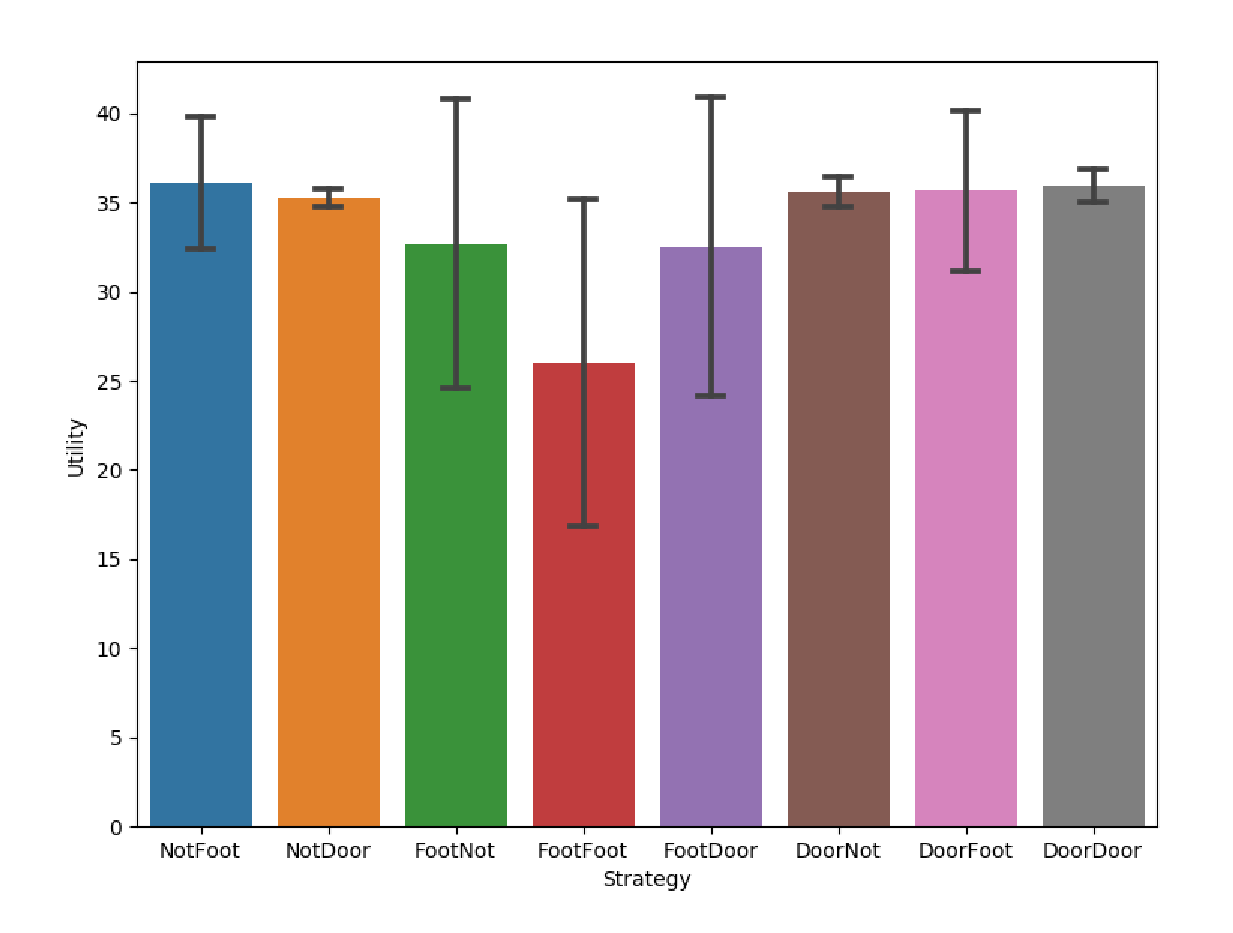
\includegraphics[width=13truecm]{image/bar_utility.eps}
  \caption{提案手法のエージェントの個人効用}
  \label{fig:pre_util}
\end{figure}

\begin{figure}[H]
  \centering
  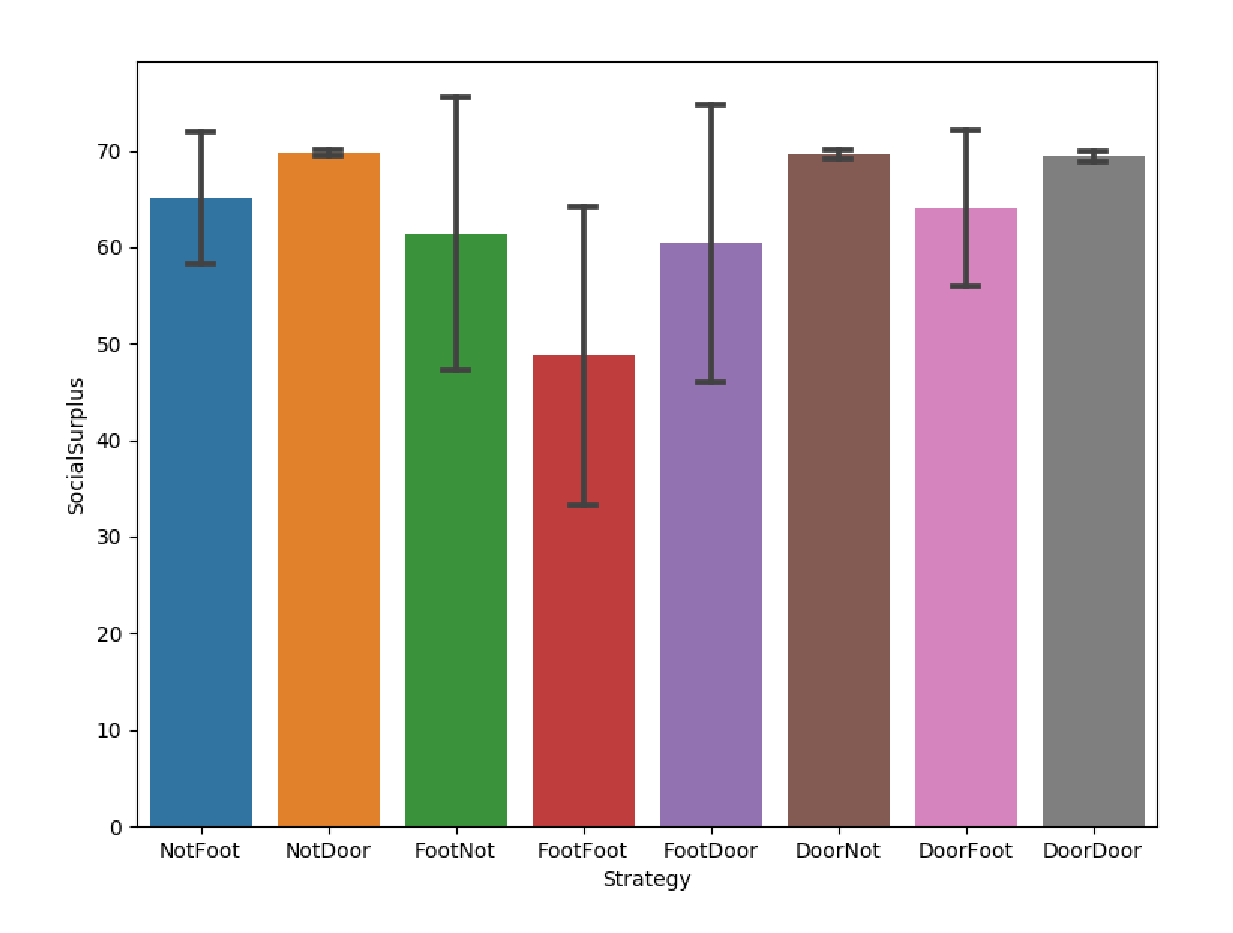
\includegraphics[width=13truecm]{image/bar_social_surplus.eps}
  \caption{エージェントの社会的余剰}
  \label{fig:pre_social}
\end{figure}

\begin{figure}[H]
  \centering
  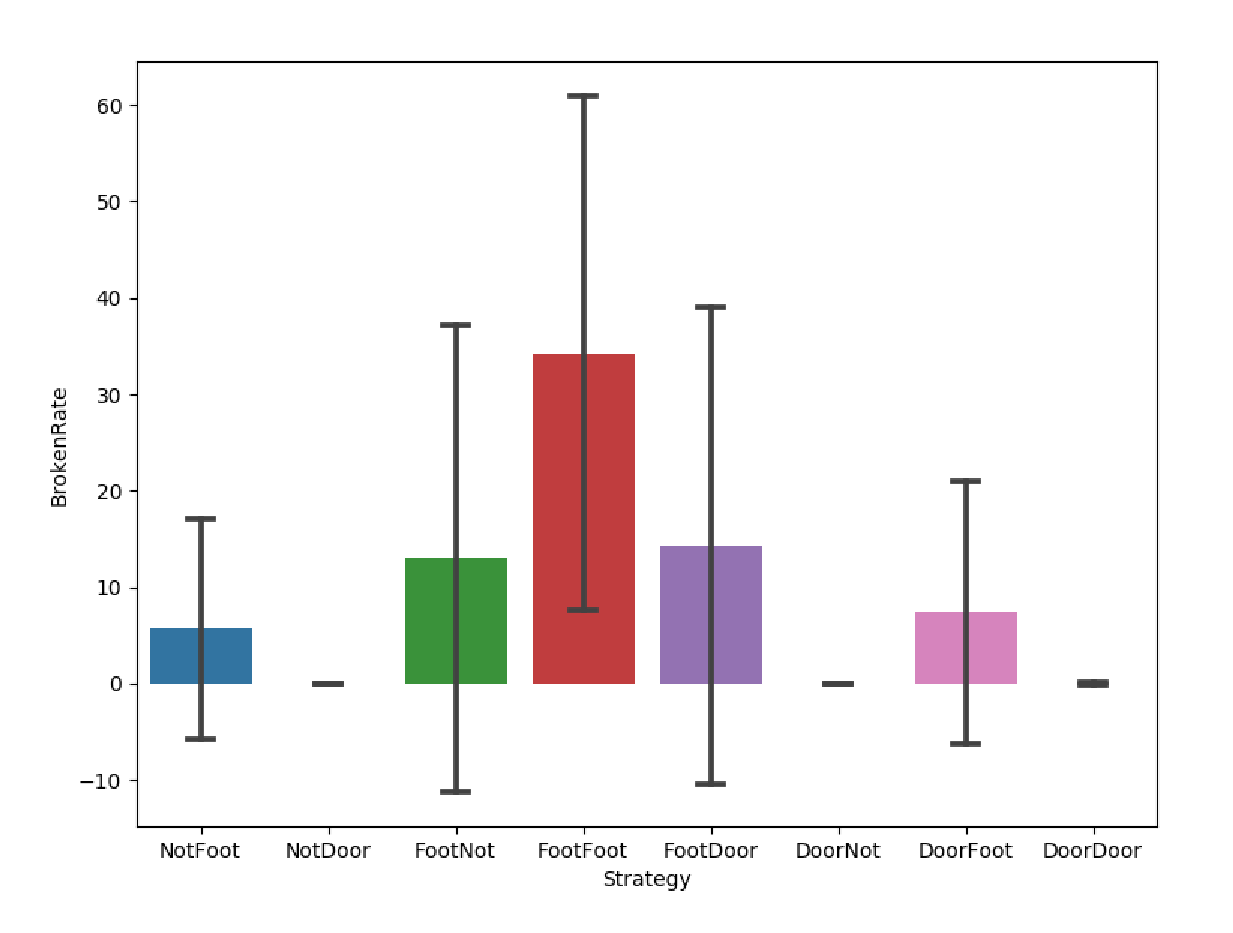
\includegraphics[width=13truecm]{image/bar_broken_rate.eps}
  \caption{提案手法のエージェントの交渉決裂率}
  \label{fig:pre_broken}
\end{figure}


図\ref{fig:pre_broken}のように,FootFootは他の戦略と比較して交渉決裂率の平均値が約$40\%$と高く,一方でNotDoor,DoorNot,DoorDoorは約$0\%$,NotFoot,DoorFootは約$5\%$,FootNot,FootDoorは約$15\%$となった.
FootFootは,相手の提案に対して自らが譲歩することがなく相手の提案を受諾する水準は単調に増加していくため,予備実験用エージェントが譲歩しても合意できない場合が多く交渉決裂率が高くなったと考えられる.FootFootは交渉決裂率が高いため,これに伴って他の戦略と比較してエージェントの個人効用および社会的余剰が低くなってしまったと考えられる.

一方のNotDoor,DoorNot, DoorDoorはいずれも交渉回数および交渉時間に応じて相手の提案を受諾する水準は単調に減少していき,予備実験用エージェントも譲歩していくため最終的にほとんどの交渉において合意に至ったと考えられる.これらの戦略は交渉が決裂することが少なかったため,FootFootと比較してエージェントの効用および社会的余剰が高くなったと考えられる.また,これらの戦略はエージェントの個人効用が平均値が約35,社会的余剰の平均値が約70となっており,分散も小さい.したがって,これらの戦略では安定して社会的余剰が最大となる合意案に達することが可能であると考えられる.

NotFoot,DoorFootはいずれも外側の戦略がFootであり,交渉時間に応じて相手の提案を受諾する水準は単調に増加していくが,内側の戦略では単調減少または変化なしである.そのため,外側の戦略が同じくFootであるFootFootと比較して交渉決裂率が低くなったと考えられる.また,これらの戦略はNotDoor,DoorNot, DoorDoorよりも交渉決裂率が高いにも関わらずエージェントの個人効用の平均値は約35である.したがって,NotFoot,DoorFootの戦略は交渉が合意に至らない可能性があるが代わりに個人効用が高くなりやすい戦略であると考えられる.

FootNot,FootDoorはいずれも内側の戦略がFootであり,交渉回数に応じて相手の提案を受諾する水準は単調に増加していくが,内側の戦略では単調減少または変化なしである.そのため,外側の戦略が同じくFootであるFootFootと比較して交渉決裂率が低くなったと考えられる.また,これらの戦略はNotFoot,DoorFootよりもエージェントの個人効用および社会的余剰の平均値が低くなっている.これは,外側の戦略では4回水準が増加するのに対して,本実験では内側の戦略は平均で5回水準が増加するからであると考えられる.したがって,水準の更新回数が多い内側の戦略にFootを用いているFootNot,FootDoorはNotFoot,DoorFootよりエージェントの個人効用および社会的余剰の平均値が低くなってしまったと考えられる.

\subsection{パラメータ\alpha の実験結果と考察}

予備実験において,パラメータ$\alpha$の増分および初期値ごとの提案手法のエージェントの効用値を図\ref{fig:a_util_1},図\ref{fig:a_util_2},図\ref{fig:a_util_3}に,交渉決裂率を図\ref{fig:a_rate_1},図\ref{fig:a_rate_2},図\ref{fig:a_rate_3}にそれぞれ示す.図\ref{fig:a_util_1},図\ref{fig:a_util_2},図\ref{fig:a_util_3}は縦軸が$\alpha$の増分,横軸が$\alpha$の初期値,色が個人効用を表しており,青に近いほど低い値,赤に近いほど高い値となる.図\ref{fig:a_rate_1},図\ref{fig:a_rate_2},図\ref{fig:a_rate_3}は縦軸が$\alpha$の増分,横軸が$\alpha$の初期値,色が交渉決裂率を表しており,青に近いほど低い値,赤に近いほど高い値となる.

\begin{figure}[H]
  \centering
  \includegraphics[width=15truecm]{image/a_util_1.eps}
  \caption{提案手法のパラメータ$\alpha$における増分・初期値に対する個人効用(1)}
  \label{fig:a_util_1}
\end{figure}

\begin{figure}[H]
  \centering
  \includegraphics[width=15truecm]{image/a_util_2.eps}
  \caption{提案手法のパラメータ$\alpha$における増分・初期値に対する個人効用(2)}
  \label{fig:a_util_2}
\end{figure}

\begin{figure}[H]
  \centering
  \includegraphics[width=15truecm]{image/a_util_3.eps}
  \caption{提案手法のパラメータ$\alpha$における増分・初期値に対する個人効用(3)}
  \label{fig:a_util_3}
\end{figure}

\begin{figure}[H]
  \centering
  \includegraphics[width=15truecm]{image/a_rate_1.eps}
  \caption{提案手法のパラメータ$\alpha$における増分・初期値に対する交渉決裂率(1)}
  \label{fig:a_rate_1}
\end{figure}

\begin{figure}[H]
  \centering
  \includegraphics[width=15truecm]{image/a_rate_2.eps}
  \caption{提案手法のパラメータ$\alpha$における増分・初期値に対する交渉決裂率(2)}
  \label{fig:a_rate_2}
\end{figure}

\begin{figure}[H]
  \centering
  \includegraphics[width=15truecm]{image/a_rate_3.eps}
  \caption{提案手法のパラメータ$\alpha$における増分・初期値に対する交渉決裂率(3)}
  \label{fig:a_rate_3}
\end{figure}

FootNot,FootDoorは$\alpha$の増分が0.5,1.0の場合は$\alpha$の初期値が高くなるにつれて個人効用は高くなり,$\alpha$の増分が1.5以上の場合は$\alpha$の初期値が高くなるにつれて個人効用が低くなった.$\alpha$の増分が低い場合は初期値が高くても相手が譲歩して合意に至ることができたと考えられる.また,$\alpha$の初期値が高い方がエージェントの受諾水準が高くなるため,$\alpha$の増分が低く初期値が高い場合に合意できたときは個人効用が高い値になったと考えられる.一方で,$\alpha$の増分が高い場合は相手が譲歩しても受諾水準が高すぎて合意に至ることができなかったと考えられる.そのため,初期値が高くなるにつれて交渉決裂率が高くなり個人効用が低くなったと考えられる.

FootFootは$\alpha$の増分および初期値が非常に低い場合のみが個人効用が高くなった.FootFootは外側の戦略にもFootを用いているため,$\alpha$の増分および初期値が低い値でないと受諾水準が高くなりすぎてしまうと考えられる.したがって,$\alpha$の増分および初期値が高い場合は交渉決裂率が非常に高くなり,その結果個人効用が低くなると考えられる.一方で,$\alpha$の増分および初期値が非常に低い場合は相手の譲歩を十分に引き出すことができないため,合意に至ったとしても個人効用がFootNot,FootDoorと比較して低くなったと考えられる.

DoorNot,DoorDoorは$\alpha$の初期値が3.0以下のとき$\alpha$の増分に関わらず個人効用はほぼ一定となり,$\alpha$の初期値が4.0以上のときは$\alpha$の増分が低いほど個人効用が高くなった.Door戦略は受諾水準を単調に減少させるため,$\alpha$の初期値が低いと受諾水準が下がりすぎてしまい,合意に至ることはできるが相手の譲歩を引き出すことができず,個人効用が低くなってしまうと考えられる.$\alpha$の初期値が高い場合であっても増分が大きい場合も同様に相手の譲歩を引き出すことができず,個人効用が低くなると考えられる.

DoorFootは$\alpha$の初期値が高く,増分が小さいほど個人効用が低くなった.DoorFootは外側の戦略にFootを用いているため,$\alpha$の初期値が高く,増分が小さい場合は受諾水準が高くなりすぎてしまい,交渉決裂率が上昇し個人効用が低くなると考えられる.それ以外の場合は,個人効用の値および交渉決裂率があまり変化していない.これはDoorNot,DoorDoorと同様の理由で受諾水準が下がりすぎてしまい相手の譲歩を引き出すことができず,個人効用が低くなると考えられる.

また,$\alpha$の更新回数ごとの提案手法のエージェントの個人効用の平均値を図\ref{fig:change_num}に示す.縦軸がエージェントの個人効用,横軸が$\alpha$の更新回数である.

\begin{figure}[H]
  \centering
  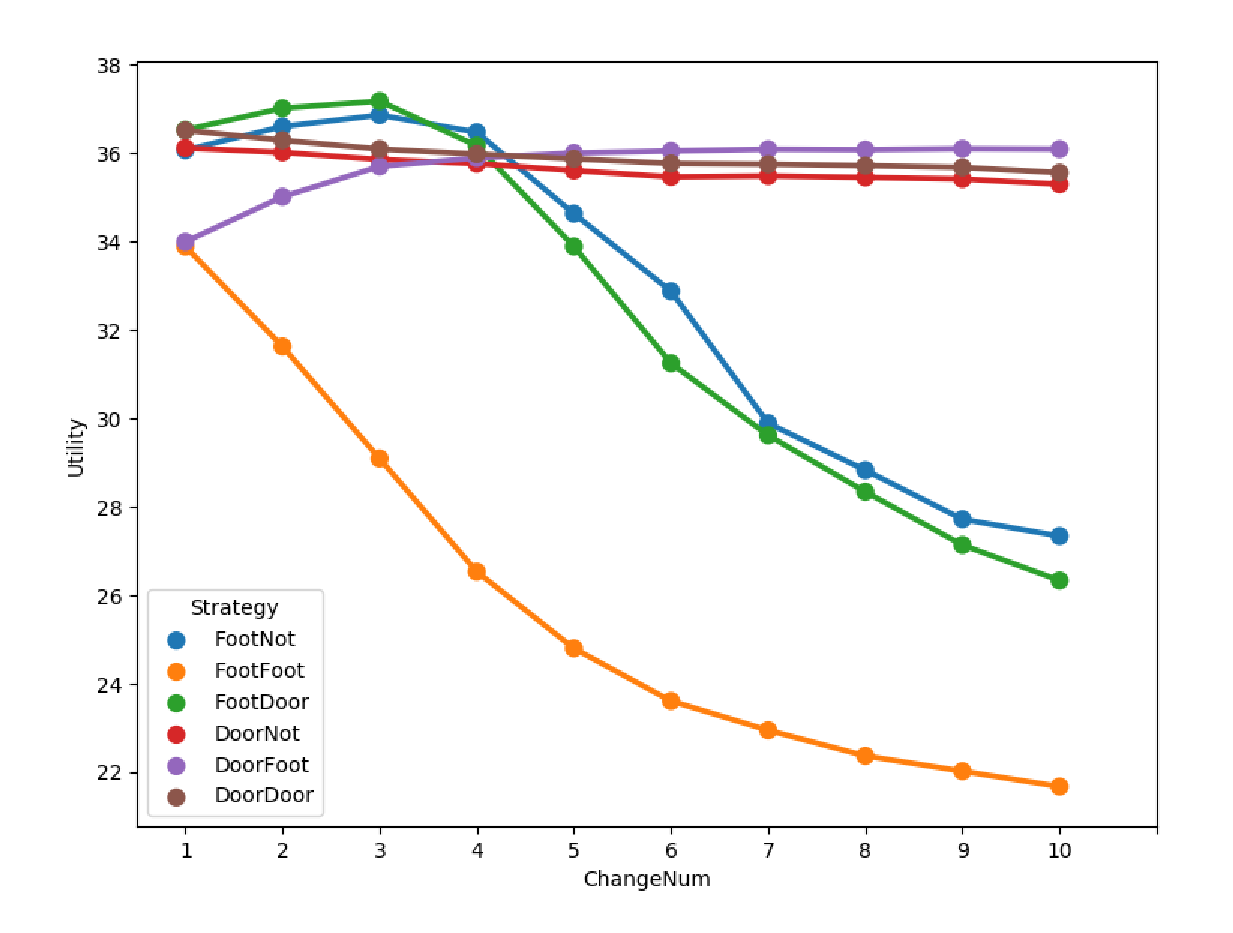
\includegraphics[width=13truecm]{image/change_num.eps}
  \caption{$\alpha$の更新回数に対する個人効用}
  \label{fig:change_num}
\end{figure}

FootNot,FootFoot,FootDoorは他の戦略と比較して$\alpha$の更新回数を変化させた場合の個人効用の変化率が高くなっている.
これらは共通して内側の戦略にFootを用いているため,$\alpha$の更新回数が多いと受諾水準が上昇し,交渉決裂率が上昇するため,個人効用が減少していったと考えられる.一方,DoorNot,DoorFoot,DoorDoorは$\alpha$が変化しても個人効用はあまり変化しなかった.これらは内側の戦略にDoorを用いているため,$\alpha$の更新回数が多いと受諾水準が下降し,相手の譲歩が引き出せなくなるが,交渉決裂率は上昇しないため,個人効用の平均値はあまり変化しなかったと考えられる.

\subsection{パラメータ\beta の実験結果と考察}

予備実験において,パラメータ$\beta$の増分および初期値ごとの提案手法のエージェントの個人効用を図\ref{fig:b_util_1},図\ref{fig:b_util_2},図\ref{fig:b_util_3}に,交渉決裂率を図\ref{fig:b_rate_1},図\ref{fig:b_rate_2},図\ref{fig:b_rate_3}にそれぞれ示す.図\ref{fig:b_util_1},図\ref{fig:b_util_2},図\ref{fig:b_util_3}は縦軸が$\beta$の増分,横軸が$\beta$の初期値,色が個人効用を表しており,青に近いほど低い値,赤に近いほど高い値となる.図\ref{fig:b_rate_1},図\ref{fig:b_rate_2},図\ref{fig:b_rate_3}は縦軸が$\beta$の増分,横軸が$\beta$の初期値,色が交渉決裂率を表しており,青に近いほど低い値,赤に近いほど高い値となる.

\begin{figure}[H]
  \centering
  \includegraphics[width=15truecm]{image/b_util_1.eps}
  \caption{提案手法のパラメータ$\beta$における増分・初期値に対する個人効用(1)}
  \label{fig:b_util_1}
\end{figure}

\begin{figure}[H]
  \centering
  \includegraphics[width=15truecm]{image/b_util_2.eps}
  \caption{提案手法のパラメータ$\beta$における増分・初期値に対する個人効用(2)}
  \label{fig:b_util_2}
\end{figure}

\begin{figure}[H]
  \centering
  \includegraphics[width=15truecm]{image/b_util_3.eps}
  \caption{提案手法のパラメータ$\beta$における増分・初期値に対する個人効用(3)}
  \label{fig:b_util_3}
\end{figure}

\begin{figure}[H]
  \centering
  \includegraphics[width=15truecm]{image/b_rate_1.eps}
  \caption{提案手法のパラメータ$\beta$における増分・初期値に対する交渉決裂率(1)}
  \label{fig:b_rate_1}
\end{figure}

\begin{figure}[H]
  \centering
  \includegraphics[width=15truecm]{image/b_rate_2.eps}
  \caption{提案手法のパラメータ$\beta$における増分・初期値に対する交渉決裂率(2)}
  \label{fig:b_rate_2}
\end{figure}

\begin{figure}[H]
  \centering
  \includegraphics[width=15truecm]{image/b_rate_3.eps}
  \caption{提案手法のパラメータ$\beta$における増分・初期値に対する交渉決裂率(3)}
  \label{fig:b_rate_3}
\end{figure}

NotFoot,DoorFootは$\beta$の増分が1.5から2.0以下の場合は$\beta$の初期値が高くなるにつれて個人効用は高くなり,$\beta$の増分が2.0から2.5以上の場合は$\beta$の初期値が高くなるにつれて個人効用が低くなった.$\beta$の増分が低い場合は初期値が高くても相手が譲歩して合意に至ることができたと考えられる.また,$\beta$の初期値が高い方がエージェントの受諾水準が高くなるため,$\beta$の増分が低く初期値が高い場合に合意できたときは個人効用が高い値になったと考えられる.一方で,$\beta$の増分が高い場合は相手が譲歩しても受諾水準が高すぎて合意に至ることができなかったと考えられる.そのため,初期値が高くなるにつれて交渉決裂率が高くなり個人効用が低くなったと考えられる.

FootFootは$\beta$の増分および初期値が非常に低い場合のみが個人効用が高くなった.FootFootは内側の戦略にもFootを用いているため,$\beta$の増分および初期値が低い値でないと受諾水準が高くなりすぎてしまうと考えられる.したがって,$\beta$の増分および初期値が高い場合は交渉決裂率が非常に高くなり,その結果個人効用が低くなると考えられる.一方で,$\beta$の増分および初期値が非常に低い場合は相手の譲歩を十分に引き出すことができないため,合意に至ったとしても個人効用がNotFoot,DoorFootと比較して低くなったと考えられる.

NotDoor,DoorDoorは$\beta$の初期値が3.0以下のとき$\beta$の増分に関わらず個人効用はほぼ一定となり,$\beta$の初期値が4.0以上のときは$\beta$の増分が低いほど個人効用が高くなった.Door戦略は受諾水準を単調に減少させるため,$\beta$の初期値が低いと受諾水準が下がりすぎてしまい,合意に至ることはできるが相手の譲歩を引き出すことができず,個人効用が低くなってしまうと考えられる.$\beta$の初期値が高い場合であっても増分が大きい場合も同様に相手の譲歩を引き出すことができず,個人効用が低くなると考えられる.

FootDoorは$\beta$の初期値が高く,増分が小さいほど個人効用が低くなった.FootDoorは内側の戦略にFootを用いているため,$\beta$の初期値が高く,増分が小さい場合は受諾水準が高くなりすぎてしまい,交渉決裂率が上昇し個人効用が低くなると考えられる.それ以外の場合は,個人効用の値および交渉決裂率があまり変化していない.これはNotDoor,DoorDoorと同様の理由で受諾水準が下がりすぎてしまい相手の譲歩を引き出すことができず,個人効用が低くなると考えられる.また,図\ref{fig:b_util_2}は全体的に効用の平均値があまり変化していないのに対して図\ref{fig:a_util_2}は効用の値はばらつきが大きい.このことから,FootDoorに関しては内側のパラメータによって個人効用が大きく左右されると考えられる.

%内容ここまで

\chapter*{謝辞}
本論文を執筆するにあたり,多数の方々からご指導・ご協力いただきましたことを,心より御礼申し上げます.

指導教員である藤田桂英准教授には,研究の機会を与えていただき,研究の方針に関する助言や発表練習等の
多大なるご指導や助言をいただきましたことを深く感謝いたします.

研究に関する知識のご教示に加えて,本実験の準備を行うにあたってWEBサーバを構築する際にお力添えいただいた松根鷹生様に深く感謝申し上げます.
また,藤田桂英研究室の皆様には研究に必要な知識や意見等をいただいたことを心より感謝いたします.

本実験を行うにあたってお忙しい中ご協力いただいた同期の編入生の方々,および安井貴規様がいなければ本論文は完成に至りませんでした.
心より御礼申し上げます.

最後に,様々な面で私を支えていただいた家族に,心より感謝いたします.ありがとうございました.

\bibliographystyle{plain}
\bibliography{reference}


\begin{comment}
%付録で発表論文をつけてアピールだ!!

\renewcommand{\bibname}{付録 発表論文一覧}
%\chapter{発表論文一覧}

\begin{thebibliography}{99}
\item S. Kakimoto and K. Fujita. 二者間複数論点交渉問題におけるパレートフロント推定手法の提案. Joint Agent Workshop and Symposium, 2014.
\item S. Kakimoto and K. Fujita. Estimating Pareto Fronts using Interdependency between Issues for Bilateral Multi-issue Closed Nonlinear Negotiations. Applications Knowledge and Service Technology for Life, Environment, and Sustainability workshop(KASTLES),2014.
\item S. Kakimoto and K. Fujita. 二者間非線形交渉問題におけるパレートフロント推定を利用した自動交渉エージェントの設計と評価. 情報処理学会 第177回 知能システム研究会, 2014.

\end{thebibliography}

\end{comment}

\end{document}

